\section{\scshape Experiment Setup}

%\begin{frame} 
%\center \huge \scshape Test Environment
%\end{frame}

%\begin{frame}
%  \frametitle{Test Environment}
%  \begin{itemize}
%		\item Benchmark
%		\item Data
%	  	\item PautomacEvaluator
%	  	\item Learner
%	  	\item Models
%  \end{itemize}
%\end{frame}

\begin{frame}
	\center \huge \scshape Selecting Dataset
\end{frame}

\begin{frame}
	\frametitle{Dataset}
	\begin{itemize}
		\item 48 to 12 Datasets
		\item Number of States
		\item Transition Density
		\item Number of Symbols
	\end{itemize}
\end{frame}

\begin{frame}
	\frametitle{Number of States}
		\begin{centering}
			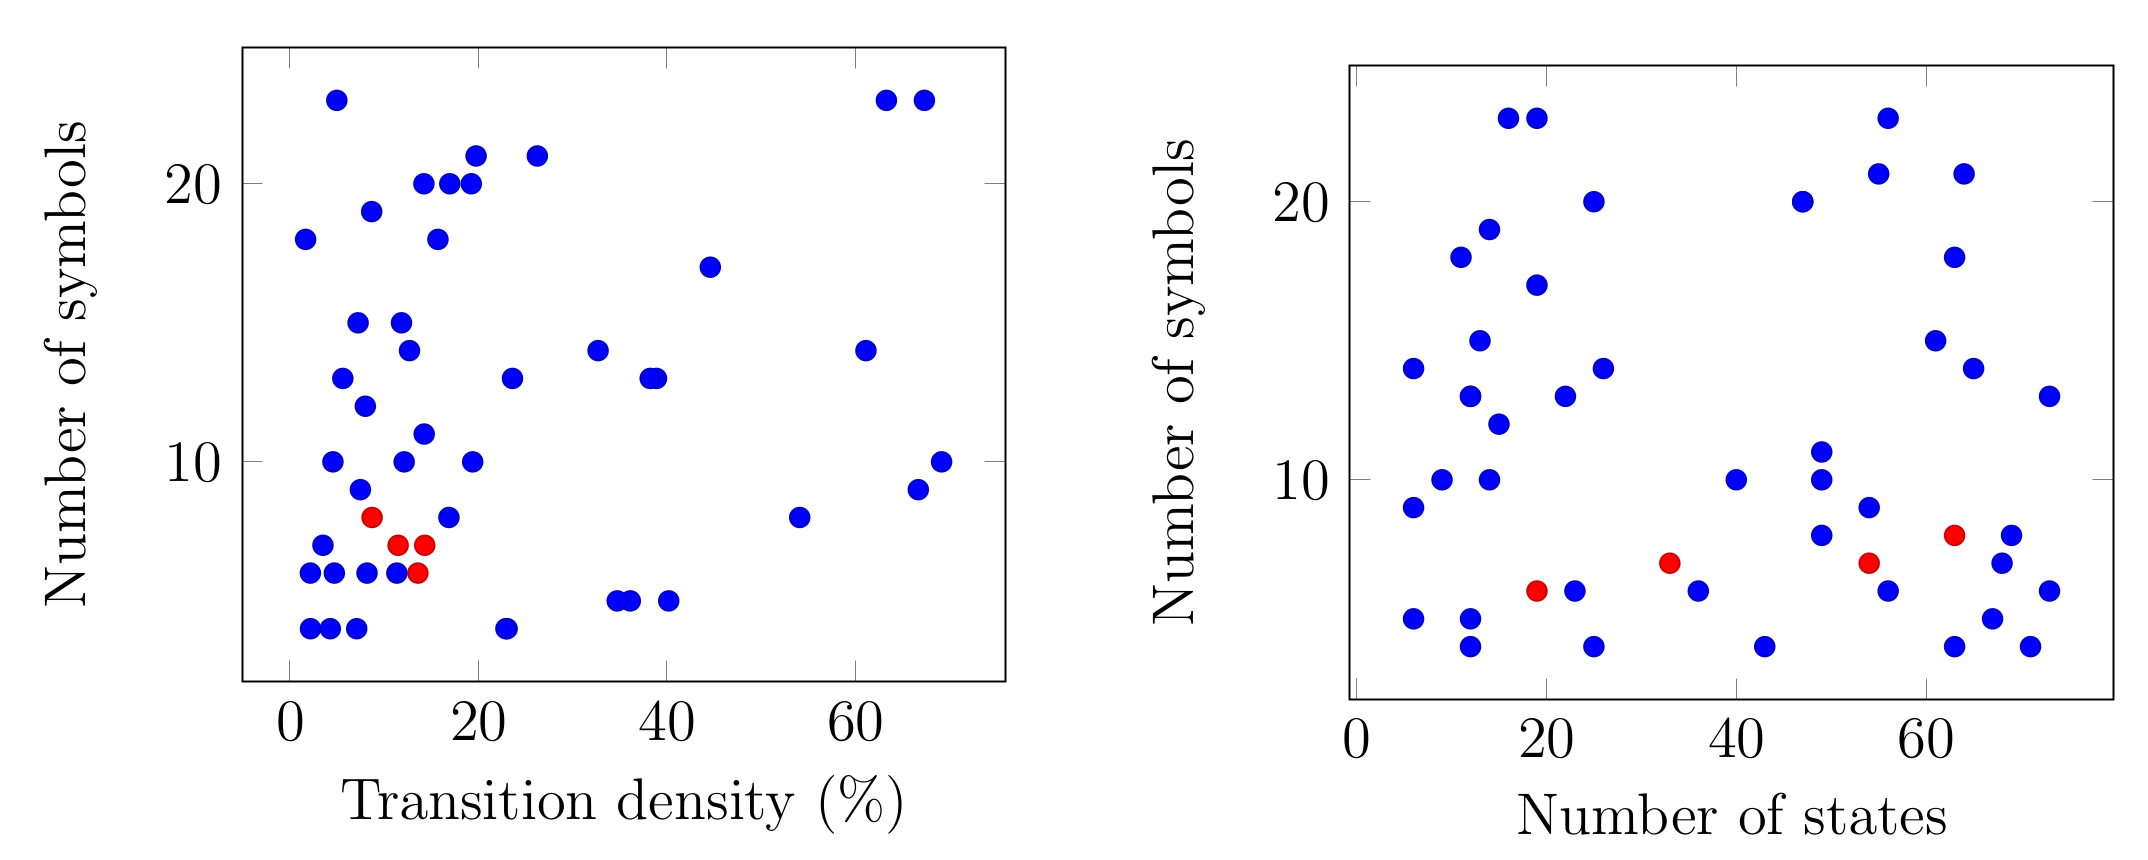
\includegraphics[width=1\textwidth]{images/states.png}
		\end{centering}
\end{frame}

\begin{frame}
	\frametitle{Transition Density}
	Ratio between number of transitions and total number of possible transitions in the model
	\begin{centering}
		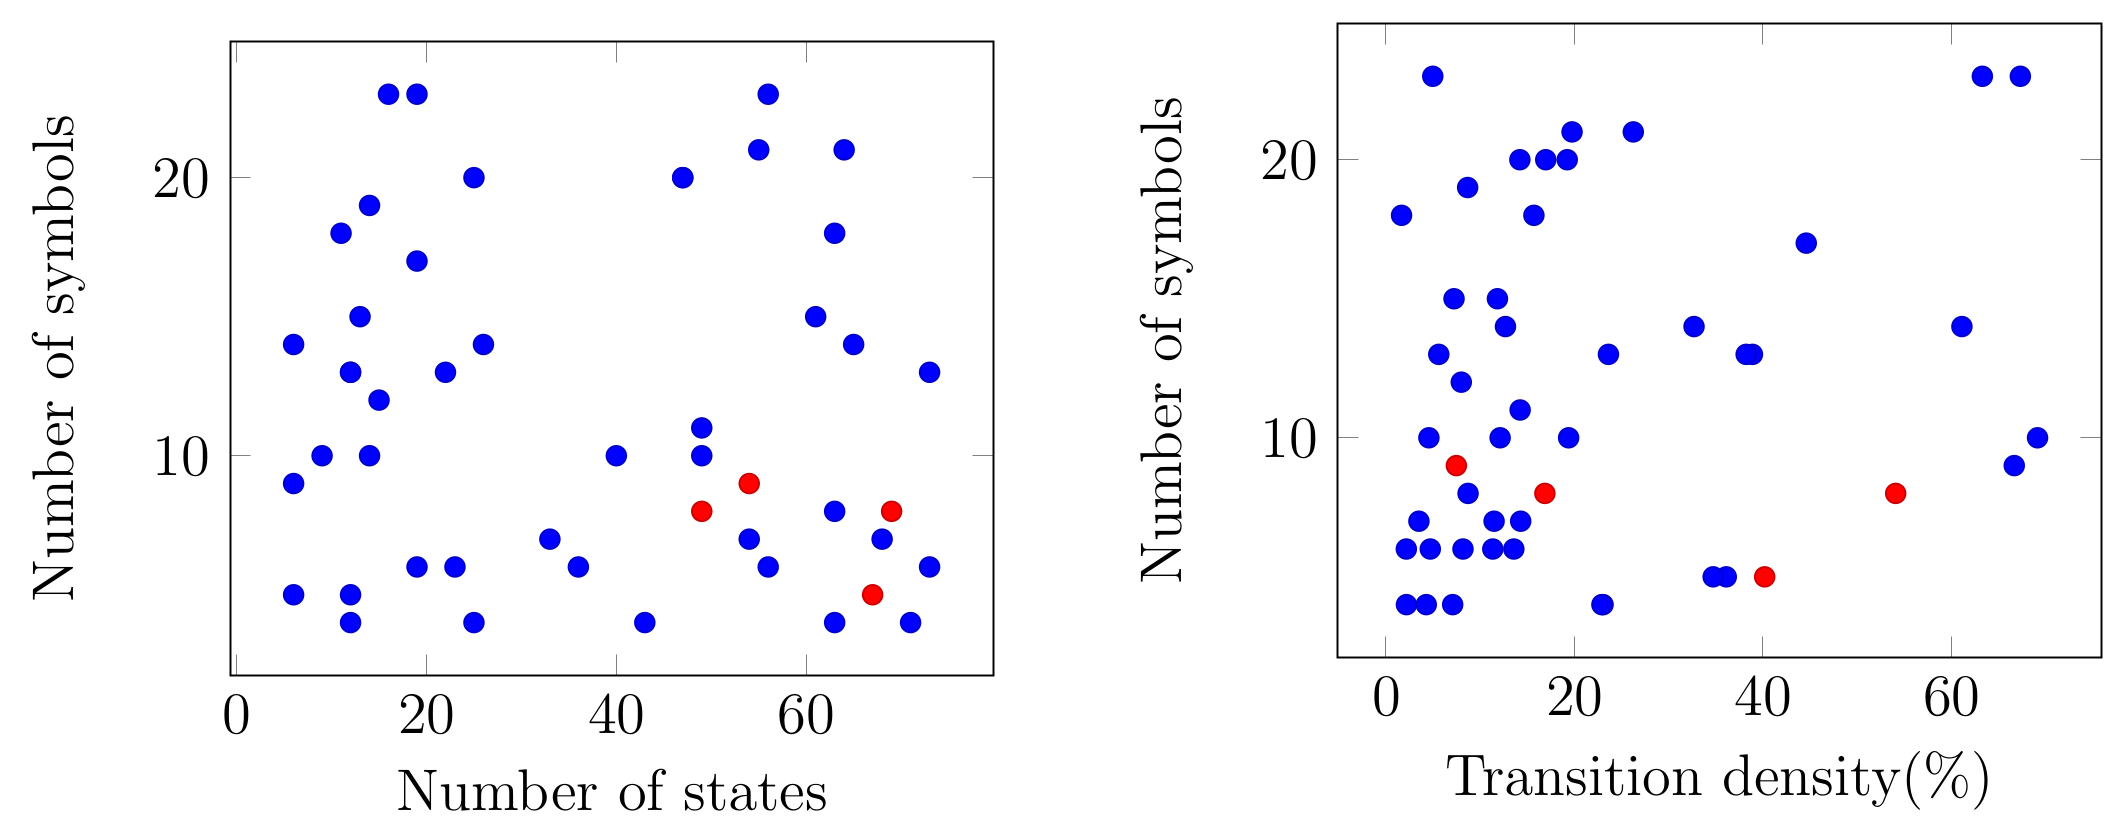
\includegraphics[width=1\textwidth]{images/transition.png}
	\end{centering}
\end{frame}

\begin{frame}
	\frametitle{Number of Symbols}
	\begin{centering}
		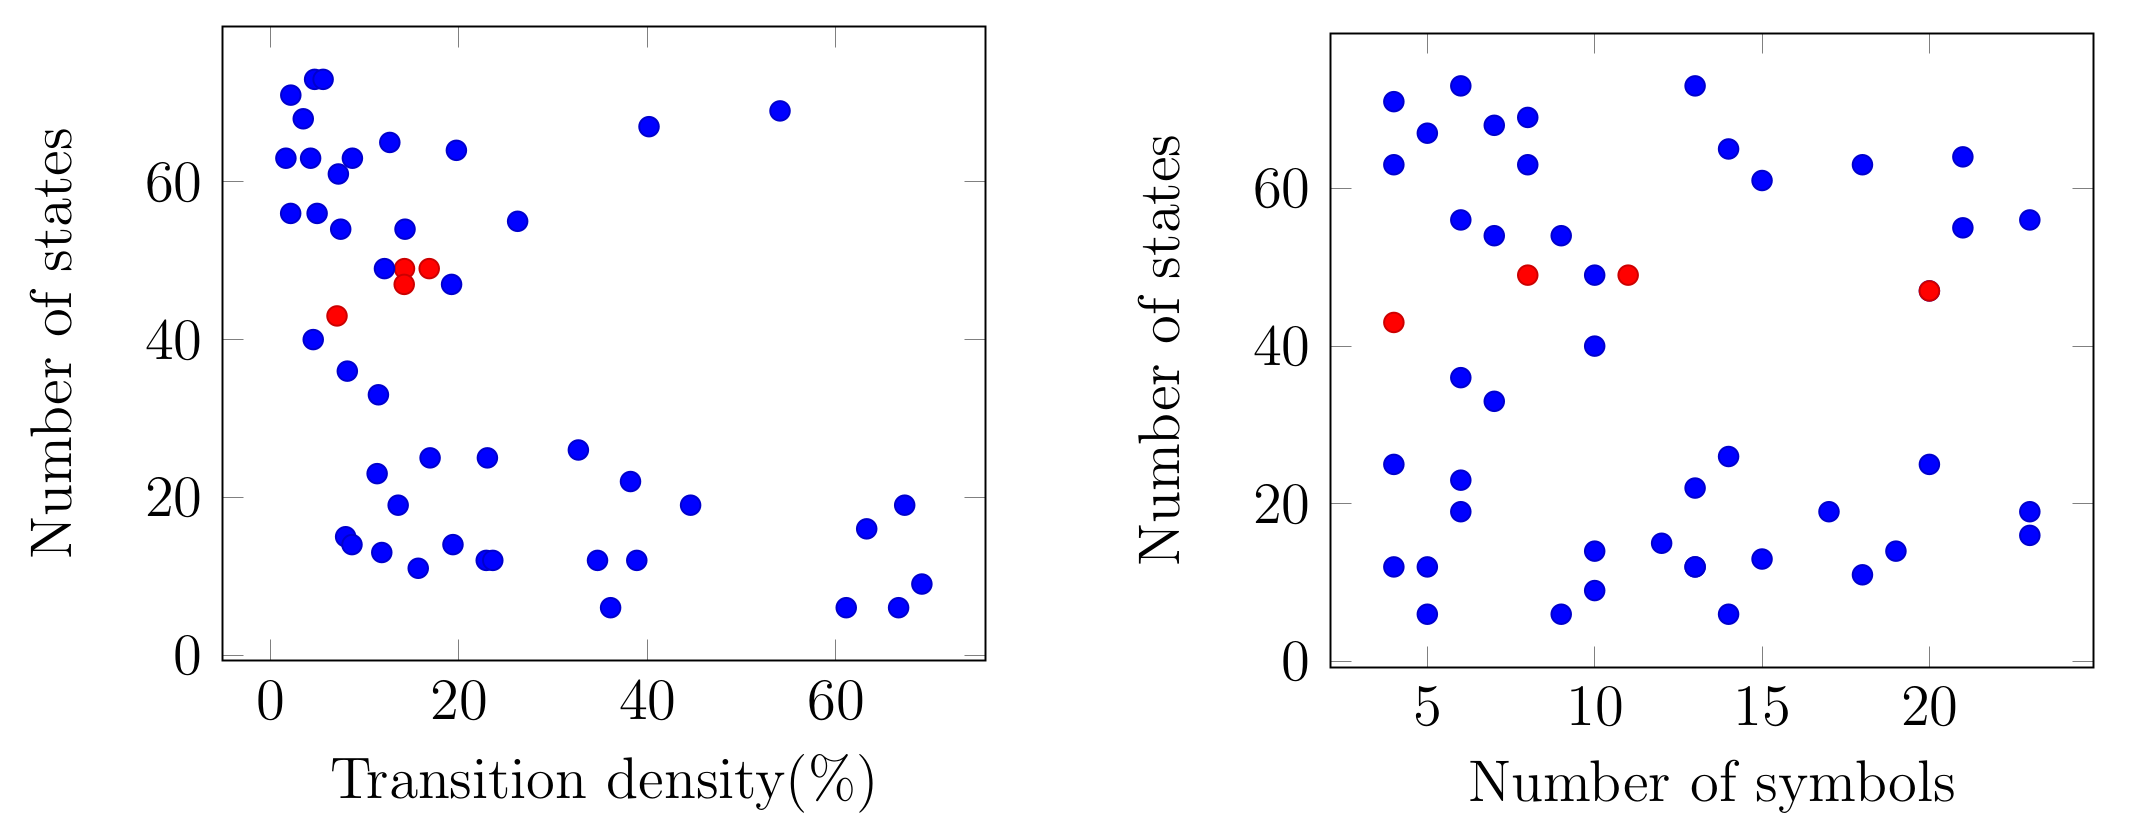
\includegraphics[width=1\textwidth]{images/symbols.png}
	\end{centering}
\end{frame}

\begin{frame}
	\frametitle{Datasets}
	\begin{centering}
		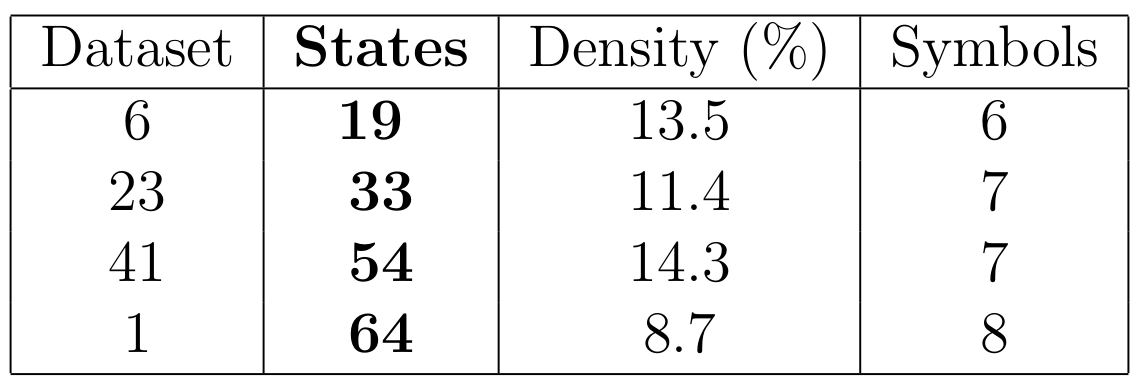
\includegraphics[width=0.7\textwidth]{images/table1.png}\\
		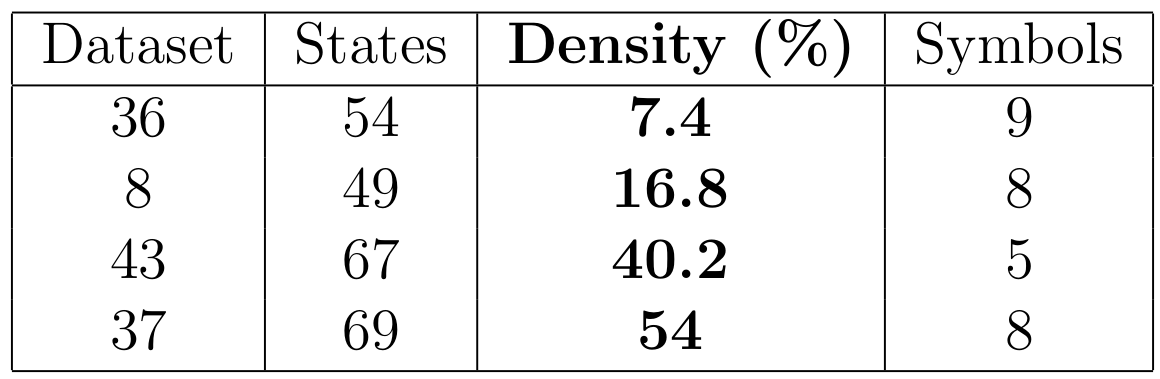
\includegraphics[width=0.7\textwidth]{images/table2.png}\\
		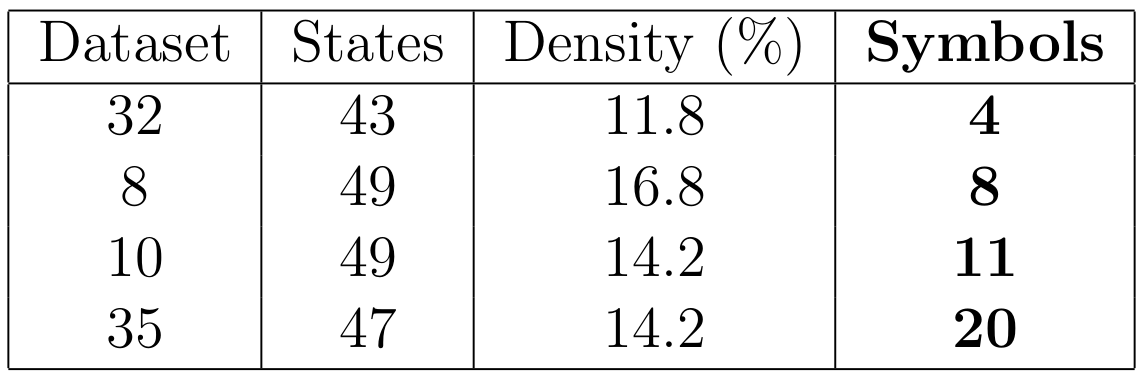
\includegraphics[width=0.7\textwidth]{images/table3.png}\\
	\end{centering}
\end{frame}

% % % % % % % % % % % % % % % % % % % % % % % % % % % % % % % %

\begin{frame}
	\center \huge \scshape Experiment Parameter
\end{frame}

\begin{frame}
	\frametitle{Experiment Parameter}
	\begin{itemize}
		\item Static Learners
		\item Training Sequences
		\item Baum-Welch Threshold
		\item Greedy Extend
	\end{itemize}
\end{frame}


\begin{frame}
	\frametitle{Static Learners}
	\begin{itemize}
		\item Baum-Welch input
		\item States for the HMM
		\item Threshold
		\item Maximum 73 states
		\item 10 to 100 step 10
	\end{itemize}
\end{frame}


\begin{frame}
	\frametitle{Training Sequences}
		\begin{itemize}
			\item 100 to 50000
			\item Baum Welch
			\item Dataset 36
			\item Threshold = 0.01
		\end{itemize}
\end{frame}

\begin{frame}
	\frametitle{Training Sequences}
	\begin{itemize}
		\item 5000 Sequences
	\end{itemize}
	\begin{centering}
		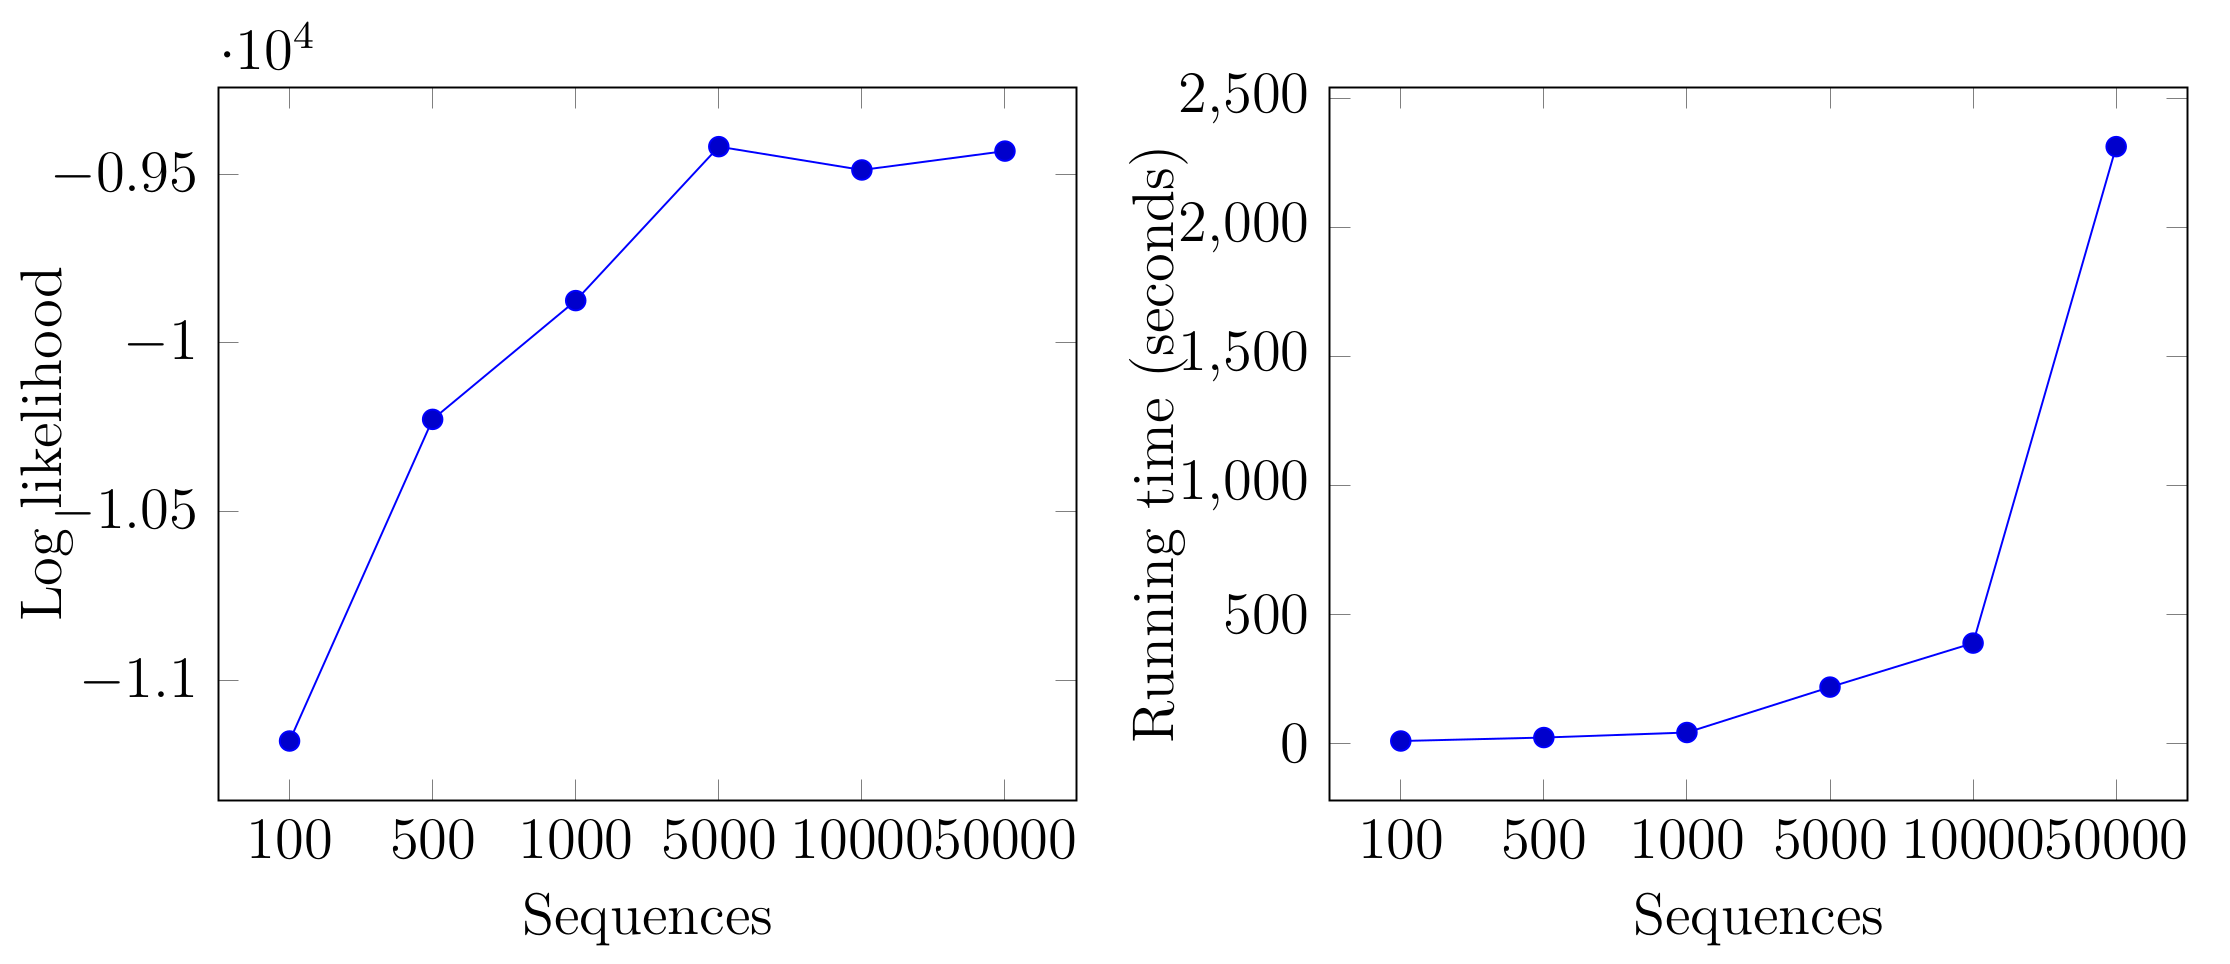
\includegraphics[width=1\textwidth]{images/sequences.png}
	\end{centering}
\end{frame}

\begin{frame}
	\frametitle{Baum-Welch Threshold}
	\begin{columns}[t]
		\begin{column}{3.3cm}
			\begin{itemize}
				\item Static value
				\item 50 states
				\item 0.1 to 0.0001
				\item Threshold 0.01
			\end{itemize}
		\end{column}
		\begin{column}{12cm}
			\begin{flushleft}			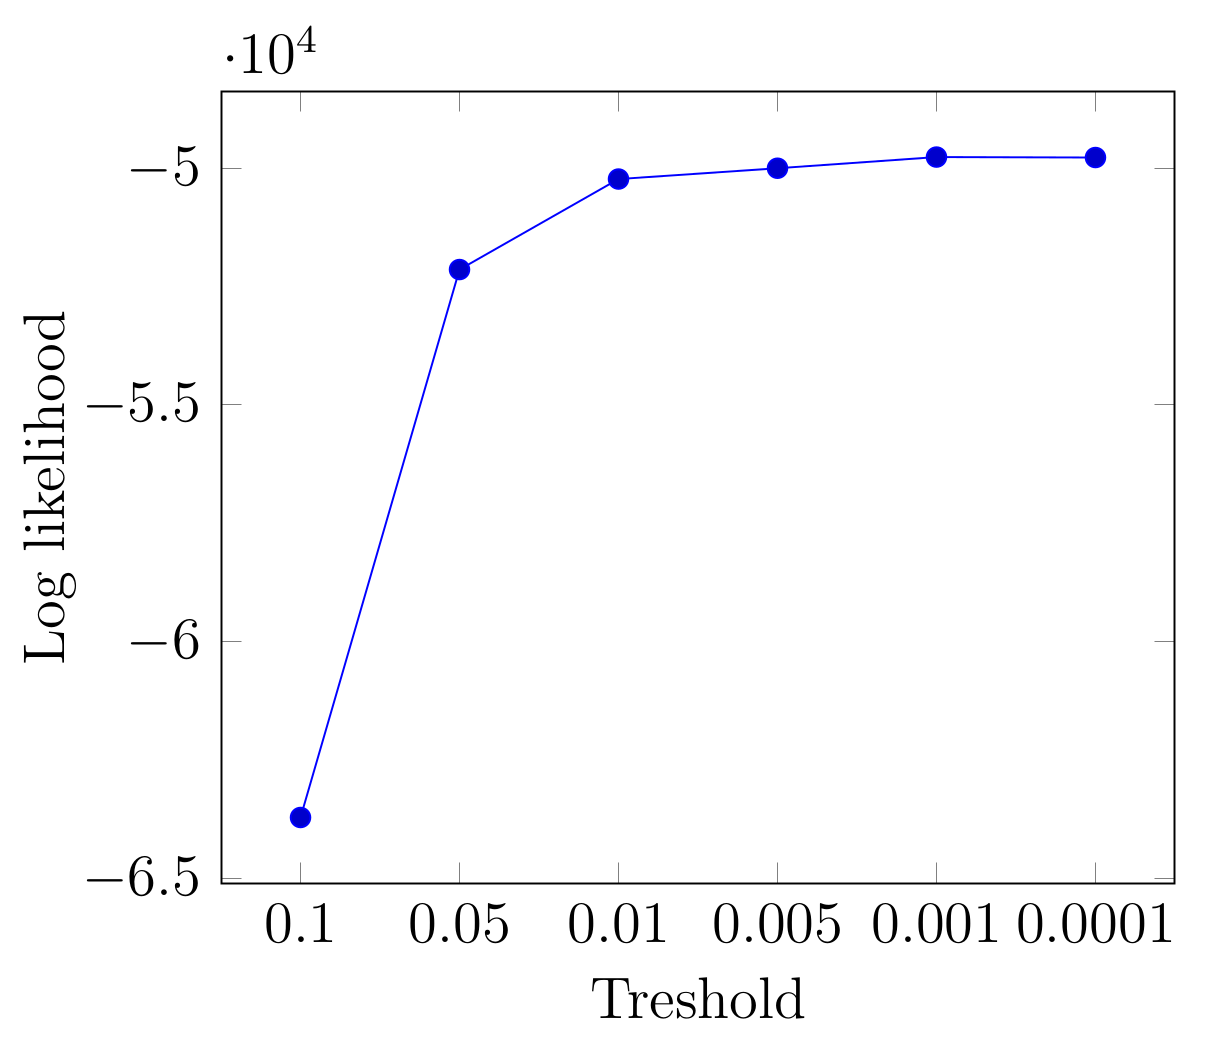
\includegraphics[width=0.7\textwidth]{images/threshold.png}
			\end{flushleft}
		\end{column}
	\end{columns}
	
\end{frame}

\begin{frame}
	\frametitle{Greedy Extend}
	\begin{itemize}
		\item $\beta$-value
		\item Baum-Welch iteration
		\item Running time
		\item Local optimum
	\end{itemize}
\end{frame}

\begin{frame}
	\frametitle{Greedy Extend}
	\begin{centering}
		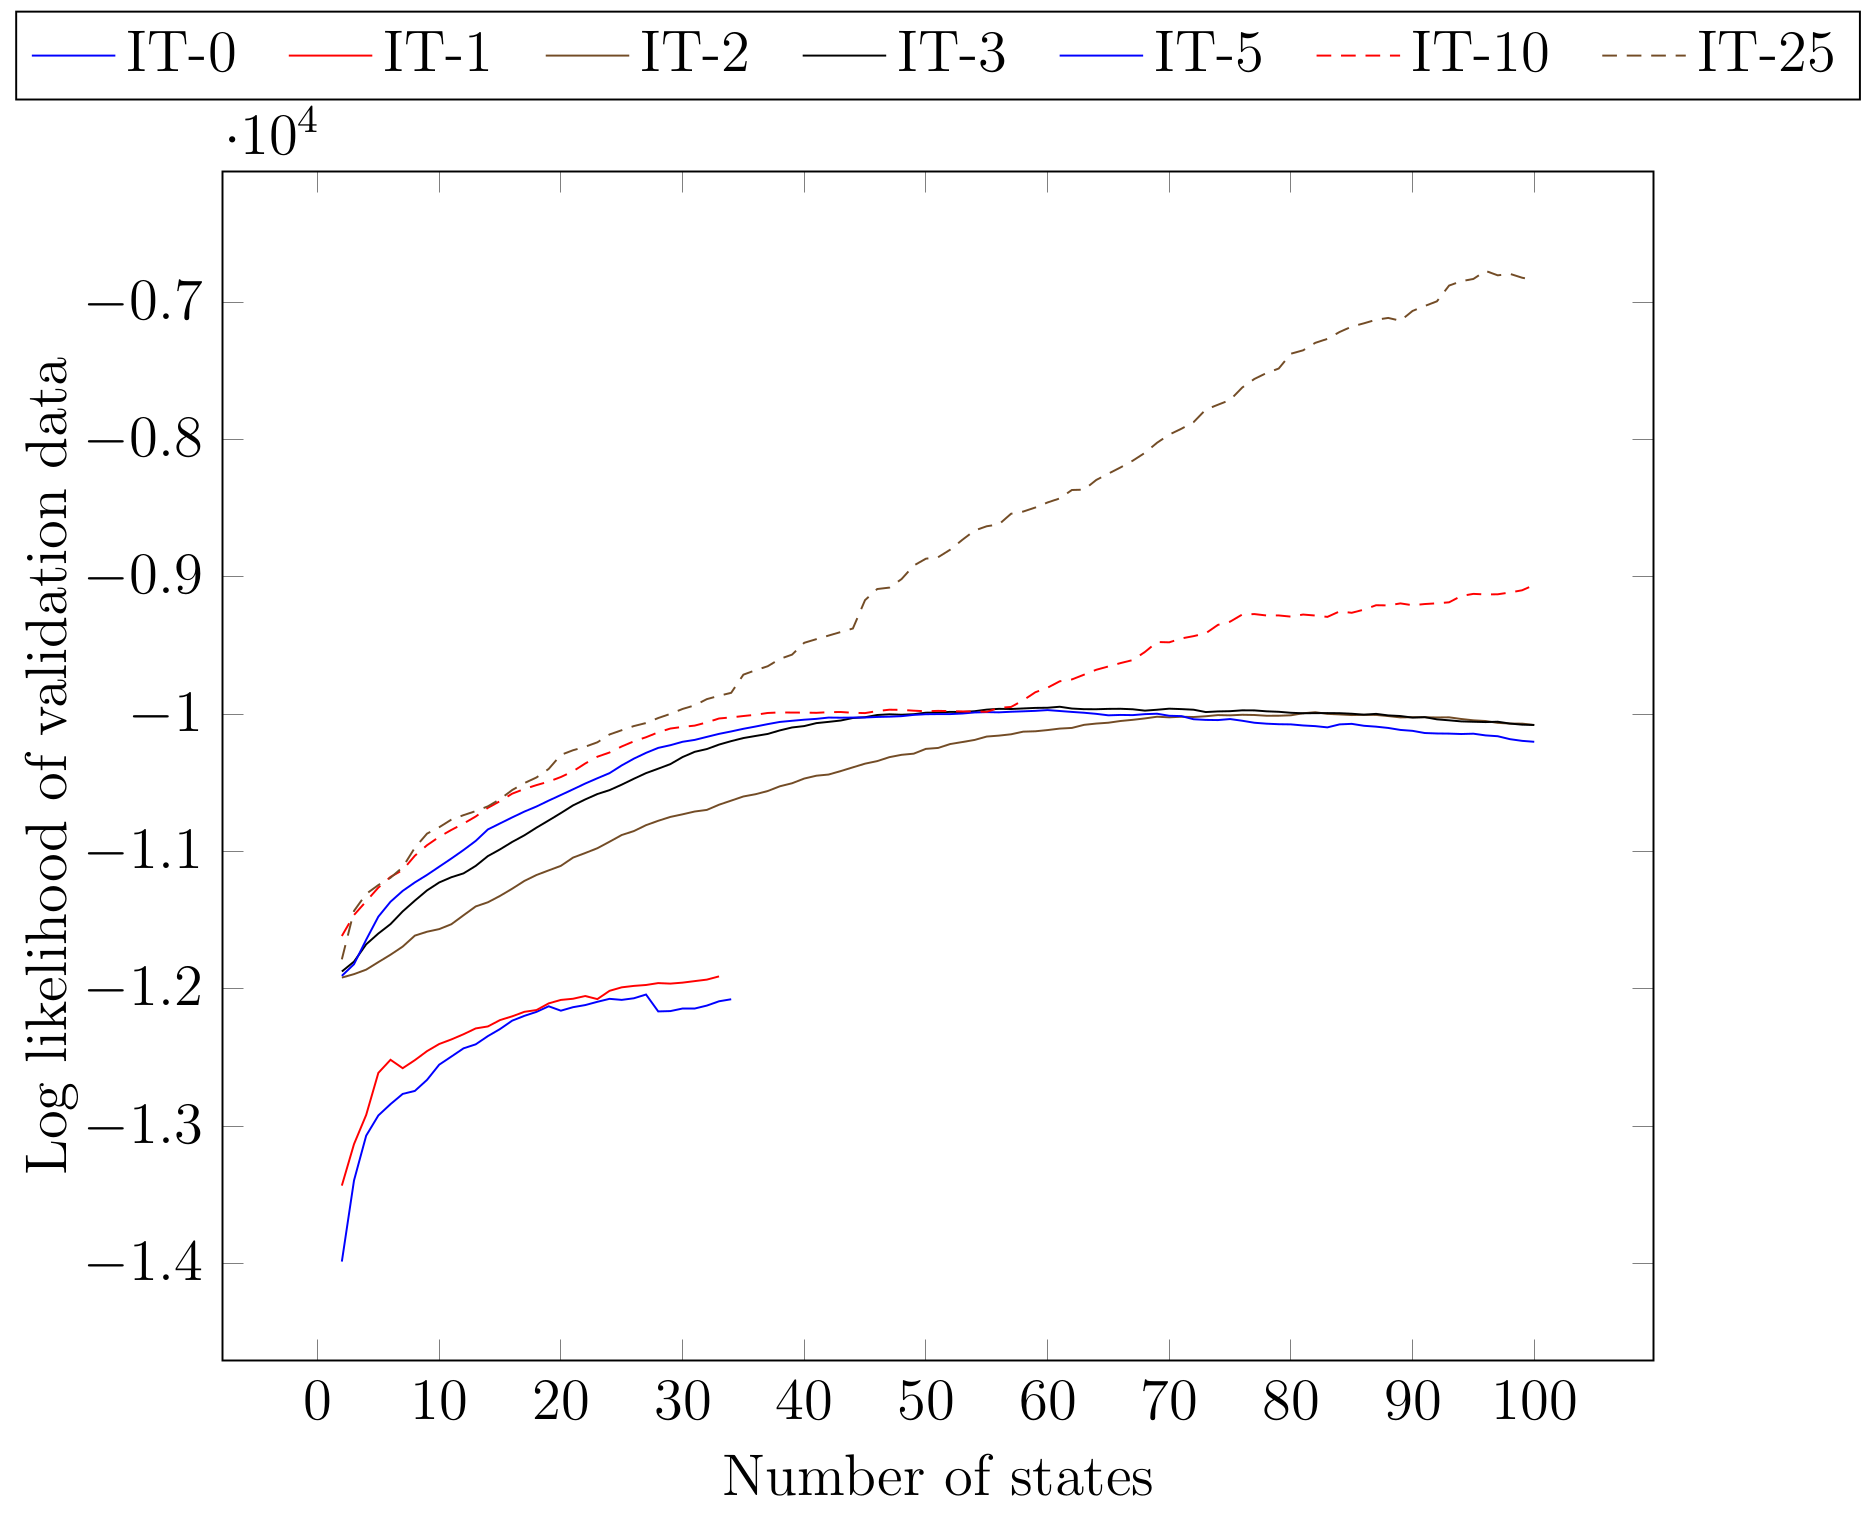
\includegraphics[width=0.9\textwidth]{images/beta.png}
	\end{centering}
\end{frame}
